
This chapter describes the implementation details of all modules in the Yoga AI Pose Detection and Correction Platform.

\section{Module Architecture and Organization}
The project is organized into several modular Python files, each handling a specific responsibility. This modular design ensures that the system is maintainable and that individual components can be tested in isolation.

The \texttt{config.py} module serves as the central repository for all configuration parameters. This includes file paths for the model and assets, hyperparameters for the training process, UI color constants, and camera settings. By centralizing these values, we can easily tune the application's behavior without modifying the core logic.

The \texttt{model.py} module defines the MobileNetV2-based transfer learning architecture. It includes the code for stripping the top layer of the pre-trained model and adding the custom classification head. It also provides utility functions for freezing and unfreezing layers during the two-stage training process.

The \texttt{train.py} script is responsible for the end-to-end training pipeline. It handles data loading, augmentation, and the execution of the two training stages. It also includes the logic for exporting training history and saving the best-performing model weights.

The \texttt{evaluate.py} script provides tools for measuring the model's performance on the test set. It generates key metrics such as precision and recall, as well as visualizations like the confusion matrix and sample prediction grids.

The \texttt{pose\_estimator.py} module encapsulates the interaction with the MediaPipe Tasks API. It handles the extraction of skeletal landmarks, the application of EMA smoothing, and the calculation of joint angles. It also contains the OpenCV-based rendering functions for the skeletal overlay.

The \texttt{pose\_rules.py} module contains the domain knowledge of the system. It defines the ideal joint angle ranges for all target poses and implements the scoring and correction logic. It also includes beginner-friendly instructions for each pose.

The \texttt{app.py} file is the main entry point of the application. It orchestrates the camera capture loop, CNN inference, the state machine logic, the voice engine, and the final HUD rendering.

\section{Data Loading and Augmentation Pipeline}
The \texttt{data\_loader.py} module builds efficient TensorFlow datasets using the \texttt{image\_dataset\_from\_directory()} utility. To ensure a robust evaluation, we reserve 15\% of the training data as a validation set.

To improve the model's ability to generalize to different camera angles and user positions, we apply several random augmentation layers to the training images. Horizontal flipping is used to handle users who may be facing either direction. Random rotation up to 10\% and random zoom of $\pm 10\%$ help the model handle slight tilts and varying distances from the camera. Furthermore, random translation of up to 10\% in both horizontal and vertical directions ensures that the model can identify poses even when they are not perfectly centered in the frame.

All images are batched with a size of 32 for stable gradient updates. Before being fed into the network, pixel values are normalized to the range $[-1, 1]$ using the \texttt{preprocess\_input} utility, aligning the data with the requirements of the pre-trained MobileNetV2 backbone.

\section{Model Training Implementation}
The training is implemented in two distinct stages to maximize the effectiveness of transfer learning.

\subsection{Stage 1: Feature Extraction Head Training}
During the first stage, the MobileNetV2 backbone is frozen to preserve its pre-trained ImageNet features. The custom classification head is trained for 10 epochs. We use the Adam optimizer with a learning rate of $10^{-3}$ and sparse categorical cross-entropy loss.
\begin{verbatim}
base_model = MobileNetV2(input_shape=(224,224,3),
                          include_top=False, weights="imagenet")
base_model.trainable = False
# Train only the custom classification head
model.compile(optimizer=Adam(lr=1e-3),
              loss="sparse_categorical_crossentropy",
              metrics=["accuracy"])
model.fit(train_ds, validation_data=val_ds, epochs=10)
\end{verbatim}

\subsection{Stage 2: Selective Backbone Fine-Tuning}
In the second stage, we unfreeze the top layers of the backbone (from layer 100 onwards) while keeping the lower layers frozen. This allows the model to learn more specialized features for yoga poses while retaining basic edge and texture detection capabilities. The learning rate is reduced to $10^{-5}$ for this stage to ensure stability.
\begin{verbatim}
for layer in base_model.layers[:100]:  # Freeze first 100 layers
    layer.trainable = False
# Unfreeze layers 100 onwards (last ~30% of MobileNetV2)
model.compile(optimizer=Adam(lr=1e-5), ...)
model.fit(train_ds, validation_data=val_ds, epochs=25)
\end{verbatim}

\section{Real-Time Pose Estimation Logic}
The \texttt{PoseEstimator} class initializes the MediaPipe landmarker using the \texttt{pose\_landmarker\_lite.task} binary. For every frame captured from the camera, the following steps are performed.

The BGR frame from OpenCV is converted to RGB and wrapped in a \texttt{mediapipe.Image}. The \texttt{detect()} method produces 33 normalized landmarks. These are then scaled to pixel coordinates based on the current frame size.

To ensure visual stability, EMA smoothing is applied to each landmark coordinate. This reduces the frame-to-frame noise inherent in the detection process. Finally, joint angles are computed using the law of cosines implementation in \texttt{calculate\_angle()}.

\subsection{Joint Angle Math Implementation}
The angle calculation function takes three landmarks—the joint vertex and two endpoints—and calculates the interior angle in degrees.
\begin{verbatim}
def calculate_angle(a, b, c):
    a, b, c = np.array(a), np.array(b), np.array(c)
    radians = np.arctan2(c[1]-b[1], c[0]-b[0]) \
            - np.arctan2(a[1]-b[1], a[0]-b[0])
    angle = np.abs(radians * 180.0 / np.pi)
    if angle > 180.0:
        angle = 360.0 - angle
    return round(angle, 1)
\end{verbatim}

\section{Corrective Logic and Scoring}
The \texttt{get\_corrections()} function implements the biomechanical evaluation. It iterates over the rules defined for the current target pose and checks if each measured joint angle is within the target range plus a 15-degree tolerance. Joints outside this range generate dynamic feedback messages that include the current angle and the target range. The overall correctness score is the ratio of correct joints to total joints evaluated for that pose.

\section{Asynchronous Voice Engine}
To ensure that speech does not block the main video processing loop, the \texttt{VoiceEngine} runs in a separate thread. It consumes correction messages from a thread-safe queue. The engine prioritizes corrections based on the degree of deviation, ensuring that the most significant form errors are addressed first.

\section{Inference Smoothing and Visibility Logic}
To prevent classification flickering, the system uses a rolling buffer of size 10 to smooth the CNN predictions. The final classification is determined by the class with the highest average probability over the buffer.

Additionally, the system performs a full-body visibility check by monitoring the ankle landmarks tracked by MediaPipe. If the ankles are not clearly visible, the system instructs the user to step back, and pose analysis is paused to ensure accuracy.

\section{User Interface Implementation}
The HUD is implemented using OpenCV's drawing primitives. It overlays the live skeletal structure, joint markers, and specific angle values onto the video frame. Subfigures in Figure~\ref{fig:app_gui} show the resulting interface for the Tree and Warrior II poses, demonstrating the clarity and density of information provided to the user.

\begin{figure}[H]
    \centering
    \begin{subfigure}[b]{0.48\textwidth}
        \centering
        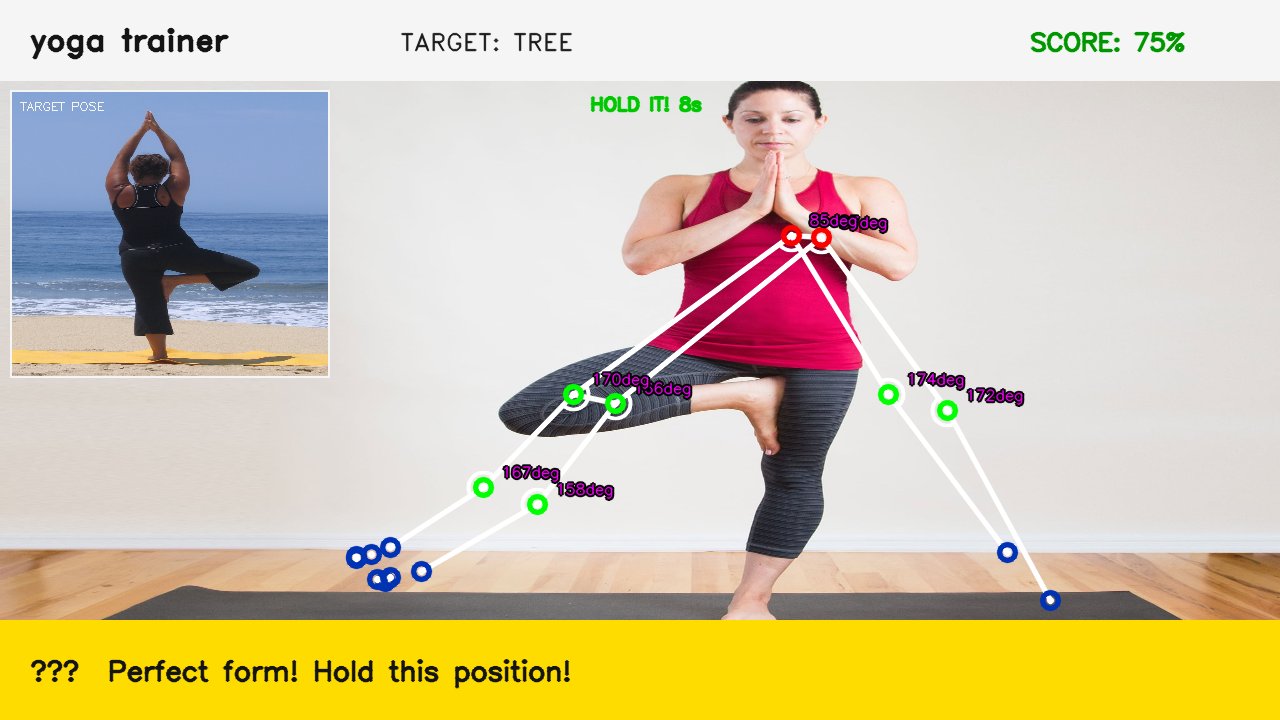
\includegraphics[width=\textwidth]{report_file/output_tree.png}
        \caption{Tree Pose HUD}
    \end{subfigure}
    \hfill
    \begin{subfigure}[b]{0.48\textwidth}
        \centering
        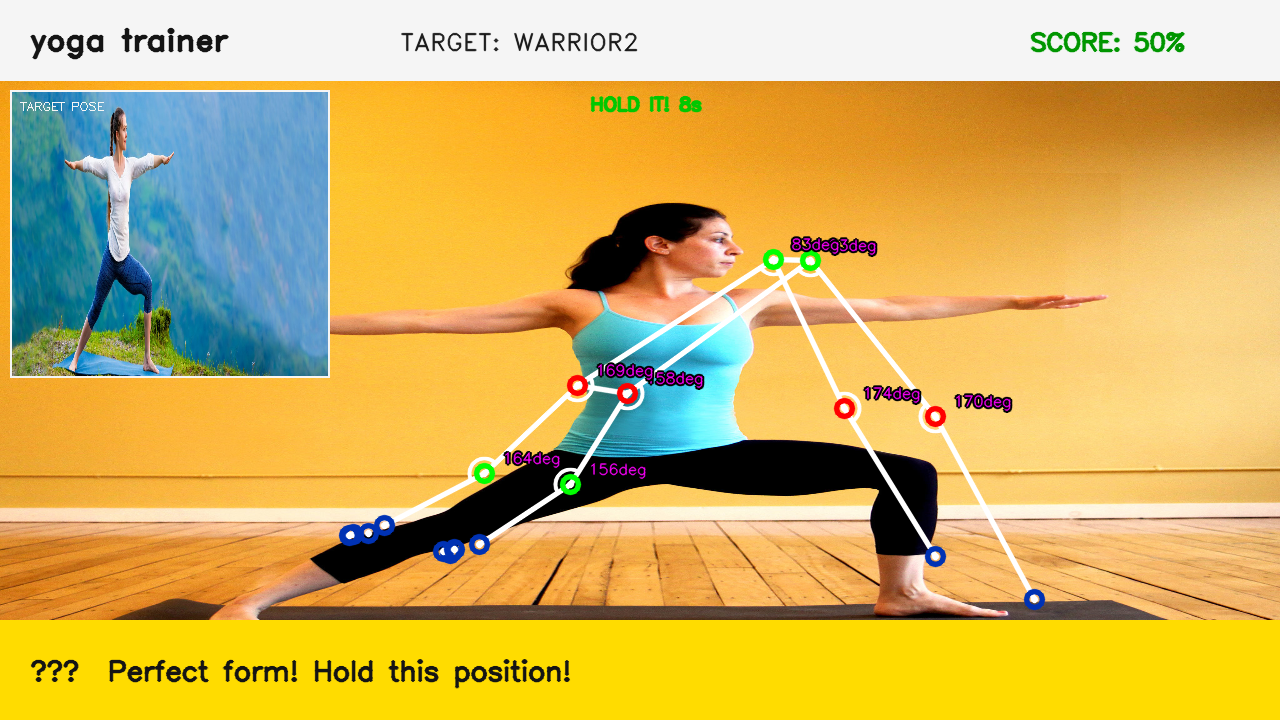
\includegraphics[width=\textwidth]{report_file/output_warrior2.png}
        \caption{Warrior II HUD}
    \end{subfigure}
    \caption{Application User Interface and Real-Time HUD}
    \label{fig:app_gui}
\end{figure}

\section{Key Engineering Challenges}
Several technical hurdles were encountered and resolved during the integration of the various platform modules.

\subsection{Challenge 1: Frame-to-Frame Landmark Jitter}
\textbf{Symptom:} The skeletal overlay and computed joint angles exhibited rapid visually distracting fluctuations, even when the user was stationary.
\textbf{Root Cause:} Inherent per-frame noise in the MediaPipe landmarker detection, combined with the extreme sensitivity of trigonometric angle calculations to small pixel displacements.
\textbf{Solution:} Implemented Exponential Moving Average (EMA) smoothing in the \texttt{PoseEstimator} with $\alpha=0.10$. This temporal filter reduced jitter significantly while maintaining high responsiveness to intentional large-scale body movements.

\subsection{Challenge 2: Multi-Threading Resource Contention}
\textbf{Symptom:} The main application window would freeze or drop to sub-5 FPS when large corrective messages were spoken via the voice engine.
\textbf{Root Cause:} The \texttt{pyttsx3} engine's \texttt{runAndWait()} method is a blocking call that consumes significant CPU time, starving the OpenCV main loop of resources.
\textbf{Solution:} Moved the voice engine into a dedicated daemon thread and implemented a thread-safe message queue. This decoupled audio output from the video processing pipeline, allowing the frame rate to remain stable even during heavy feedback events.

\subsection{Challenge 3: Classification Flickering in Dynamic Environments}
\textbf{Symptom:} The detected pose name at the top of the HUD would oscillate rapidly between labels (e.g., flipping between 'Tree' and 'Goddess' 10 times per second) when the user was in an intermediate state.
\textbf{Root Cause:} Direct reliance on single-frame CNN probabilities, which are unstable during transitional body movements.
\textbf{Solution:} Implemented a temporal prediction buffer of size 10. The system now performs a weighted moving average of probabilities over time before committing to a pose label, effectively filtering out transient misclassifications.

\subsection{Challenge 4: Anchor Coordinate Scaling across Screen Aspect Ratios}
\textbf{Symptom:} Joints appeared misaligned with the user's body on certain high-definition webcams (1080p).
\textbf{Root Cause:} Scaling errors between the fixed-size CNN input (224$\times$224) and the dynamic resolution of the video stream.
\textbf{Solution:} Implemented a unified coordinate scaling utility that normalizes the landmarker's $[0,1]$ output directly to the runtime frame dimensions $(W, H)$ before any geometric or rendering operations are performed.
